%--------------------
% Packages
% -------------------
\documentclass[11pt,a4paper]{article}
\usepackage[utf8x]{inputenc}
\usepackage[english]{babel}
\usepackage[T1]{fontenc}
%\usepackage{gentium}
% \usepackage{mathptmx} % Use Times Font


\usepackage[pdftex]{graphicx} % Required for including pictures
\usepackage[swedish]{babel} % Swedish translations
\usepackage[pdftex,linkcolor=black,pdfborder={0 0 0}]{hyperref} % Format links for pdf
\usepackage{calc} % To reset the counter in the document after title page
\usepackage{enumitem} % Includes lists

\frenchspacing % No double spacing between sentences
\linespread{1.2} % Set linespace
\usepackage[a4paper, lmargin=0.1666\paperwidth, rmargin=0.1666\paperwidth, tmargin=0.1111\paperheight, bmargin=0.1111\paperheight]{geometry} %margins
%\usepackage{parskip}

\usepackage[all]{nowidow} % Tries to remove widows
\usepackage[protrusion=true,expansion=true]{microtype} % Improves typography, load after fontpackage is selected

\usepackage{lipsum} % Used for inserting dummy 'Lorem ipsum' text into the template


\usepackage{float} % to fixate images

%-----------------------
% Set pdf information and add title, fill in the fields
%-----------------------
\hypersetup{ 	
pdfsubject = {Introduction to Machine learning and Data mining},
pdftitle = {Project 1},
pdfauthor = {Nicolò Francesco Resmini - s231858}
}

%-----------------------
% Begin document
%-----------------------
\begin{document} 

\title{Introduction to Machine learning and Data mining - Project 1} % Title

% \author{Ivan Antonino Arena - s233352 \\
%  Nathan Lacour - s232062 \\
%  Nicolò Francesco Resmini - s231858  }  % Authors
 
\date{\today}

\maketitle
\begin{table}
\centering
\begin{tabular}{lllll}
 \textbf{Student} & \textbf{ID} & \textbf{§1} & \textbf{§2} & \textbf{§3} \\
 Ivan Antonino Arena & s233352 &  &  &  \\
 Nathan Lacour & s232062 &  &  &  \\
 Nicolò Francesco Resmini & s231858 &  &  & 
\end{tabular}
\end{table}



\pagebreak

\section{Dataset Description}

\subsection{Introduction}
The dataset that we selected contains data about the use of automatic rental bike; all the process is automatic as bikes are all connected to the net. Thus, it is possible to obtain a lot of interesting information about traffic (the duration of travel, starting position of the bike and its final location). Then, the rental bikes might be used as sensors that would give us knowledge about mobility in the city. \\ 
Bike-sharing rental process is highly influenced by parameters like the weather or the time of the year.
Hence in our data set, we know the number of bikes that was rented as well as when it was rented and additional weather related information.\\
However, when opening the folder containing the data files, we had to choose between 2 files: \textit{day.csv} and \textit{hour.csv}, which have the same fields, except "hour" (0 to 23) which is not available in \textit{day.csv}. Regarding that, we chose to use \textit{hour.csv} since it gives us indeed more information and interesting ones, because the time of the day may strongly influence the number of rental bikes.\\
Given the data, we will most certainly look at how the weather conditions are correlated to the number of users.
We found the data set on the website UC Irvine (link below).\\
\textit{https://archive.ics.uci.edu/dataset/275/bike+sharing+dataset}

\subsection{Previous analysis of the data}

The Bike Sharing Dataset has been cited in more than ten scientific papers (linked on the same webpage from which we downloaded the dataset), which clearly demonstrates its breadth and its utility in supporting high-quality research. Therefore, we picked two of those papers and read them carefully to understand how this dataset had been used by the authors in their works. \\
The first one is “Recurrent Neural Networks for Time Series Forecasting” by G'abor Petneh'azi (2019), which presents a recurrent neural network-based time series forecasting framework covering feature engineering, feature importances, point and interval predictions, and forecast evaluation. Briefly, RNNs are essentially neural networks with memory, so they can remember things from the past, which is obviously useful for predicting time-dependent targets. Moreover, the author disregards the available weather information, and uses time-determined features only; he encodes the cyclical features (season of year, month of year, week of year, day of week and hour of day) ,through the use the sine and cosine transformations, and he creates some binary variables, which are used to indicate if the time is afternoon, working hour, holiday, working day. Finally, to perform the value forecasts (regression) he also calculates variable importances by applying two different accuracy metrics (called R2 and MDA). In the end, the author states that he reached good results, although he admits that even this 2-year hourly bike sharing dataset is way too small to exploit the capabilities of a neural network. \\
Furthermore, the second Paper examined is “D-vine quantile regression with discrete variables” by Niklas Schallhorn, Daniel Kraus, Thomas Nagler, Claudia Czado (2017), which introduces new quantile regression (i.e. the prediction of statistical measures called conditional quantiles) approaches to handle the presence of mixed discrete-continuous data in a dataset, like ours. Indeed, for each day we have continuous covariates temperature (Celsius), wind speed (mph) and humidity (relative in \%); additionally, there is the discrete variable weather situation giving information about the overall weather with values 1 (clear to partly cloudy), 2 (misty and cloudy) and 3 (rain, snow, thunderstorm). Eventually, by applying these new methods, prediction results show some dependencies between the features like “For temperatures higher than 32 degrees Celsius, each additional degree causes a decline in bike rentals” or “Bike rentals increase up to a relative humidity of around 60\% and decrease afterwards”. \\ 
Both these papers were really helpful to gain a deeper insight into the dataset, by making us look at the dataset from a different perspective and draw inspiration for some implementations of our project.

 \subsection{Techniques}
With these data, we might be able to establish a model to estimate how much people would rent a bike on a given day with given weathers conditions. This could indeed be useful for the people in charge of managing the city accommodations or planning events.

\begin{itemize}

\item Regression: \\
 1) Input : holyday/working day?, month/season, hour,date, weather
    Output : number of users (casual, registered or total)
    we have only two years so month might not be good since we only have 2 time each month

    
    transformation continuous ?
    
    \item  Classification: \\
 1) Input : windspeed, temperature, number of users, humidity \\
    Output : Weather
    
 2) Input : windspeed, temperature, number of users, humidity, weather \\
    Output : season
    
 3) Input :
    Ouput : month  \\
    we have only two years so month might not be good since we only have 2 time each month, a better option could be the day of the weeks.
 
\end{itemize}


    
   

    
\section{Attributes of the data}

\subsection{Attributes list}


\begin{itemize}
    \item \textbf{instant}: discrete, interval;
    \item \textbf{dteday}: discrete, interval;
    \item \textbf{season}: discrete, nominal;
    \item \textbf{yr}: discrete, nominal;
    \item \textbf{mnth}: discrete, nominal;
    \item \textbf{hr}: discrete, interval; 
    \item \textbf{holiday}: discrete, nominal;
    \item \textbf{weekday}: discrete, nominal;
    \item \textbf{workingday}: discrete, nominal;
    \item \textbf{wheatersit}: discrete, ordinal;
    \item \textbf{temp}: continous, ratio;
    \item \textbf{atemp}: continous, ratio;
    \item \textbf{hum}: continous, ratio;
    \item \textbf{windspeed}: continous, ratio;
    \item \textbf{casual}: discrete, ratio;
    \item \textbf{registered}: discrete, ratio;
    \item \textbf{cnt}: discrete, ratio;
\end{itemize}

\subsection{Data issues}

After carefully analyzing the dataset, we can confidently say that there are no missing values or corrupted data, therefore no statistical techniques to replace eventual missing values with reasonable approximations should be performed; to verify, the same conclusion has been reached in the paper “VINE: Visualizing Statistical Interactions in Black Box Models” by Matthew Britton (2019).

\subsection{Summary statistics}

\begin{figure}[H]
    \centering
    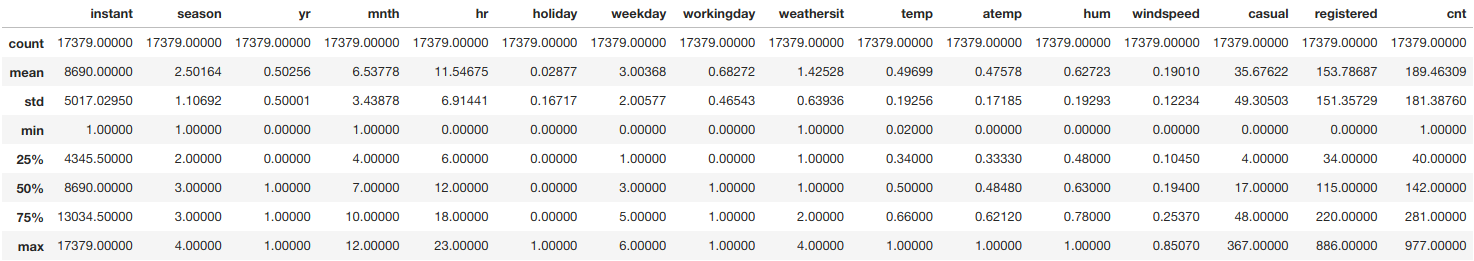
\includegraphics[width=\textwidth, height=0.3\textwidth]{res/summary.png}
    \caption{Summary statistics for the dataset.}
    \label{fig:summary}
\end{figure}



\section{Data visualization and PCA}

\subsection{Outliers}

By plotting all data in a box plot we can clearly see that the only outliers seem to be on the attributes $holiday$ and $weathersit$; however this attributes are respectively nominal and ordinal and only take two and four values, therefore we could ignore the $holiday$ attribute, since the number of holidays is negligible and convert all the entries with value $= 4$ in the $weathersit$ attribute to the value $= 3$, for the same reason. In this way, all outliers value will be taken care of.

\begin{figure}[H]
    \centering
    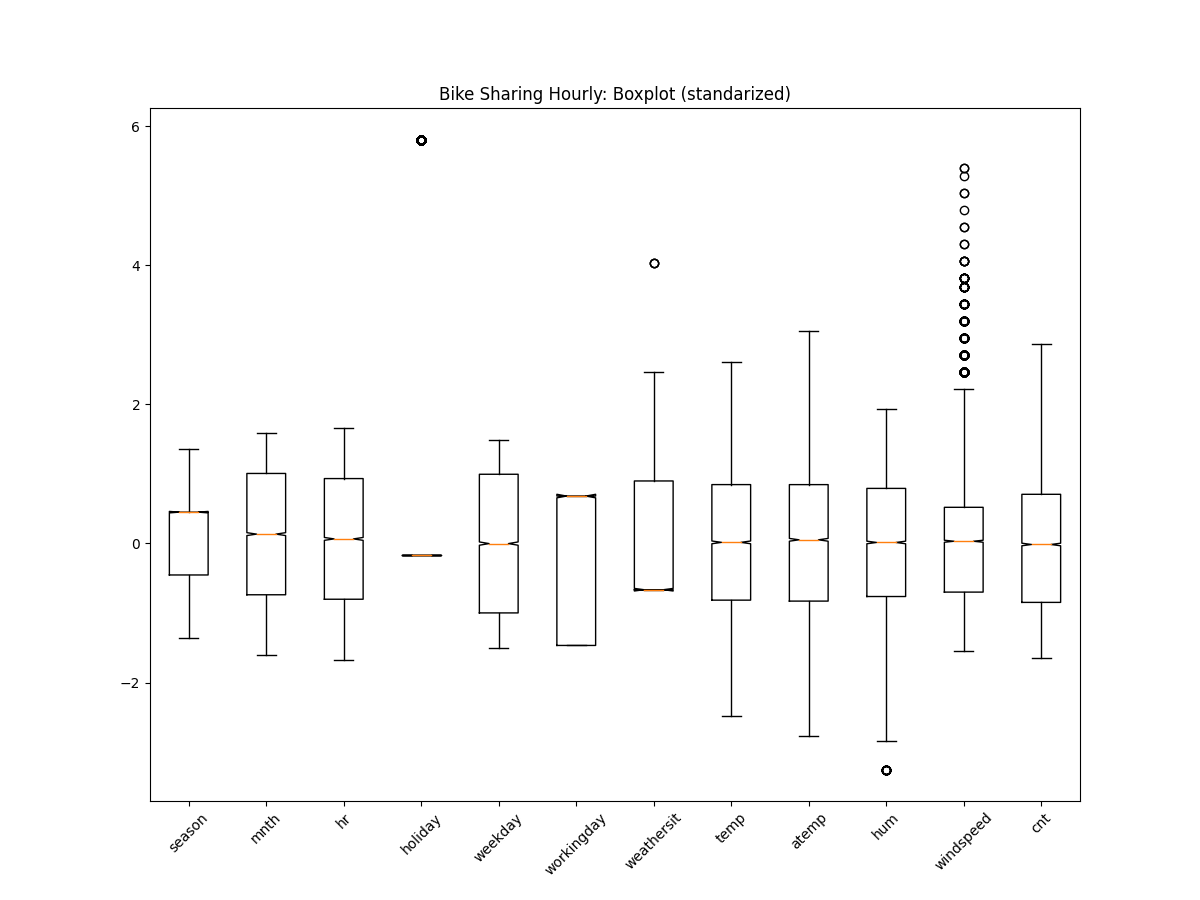
\includegraphics[width=\linewidth]{res/plots/boxplot_standardized.png}
    \caption{Standardized boxplot of the dataset.}
    \label{fig:boxplot}
\end{figure}



% you can't really see in weathersit hist that 4 has 3 values, should we modify the plot?

\begin{figure}[H]
    \centering
    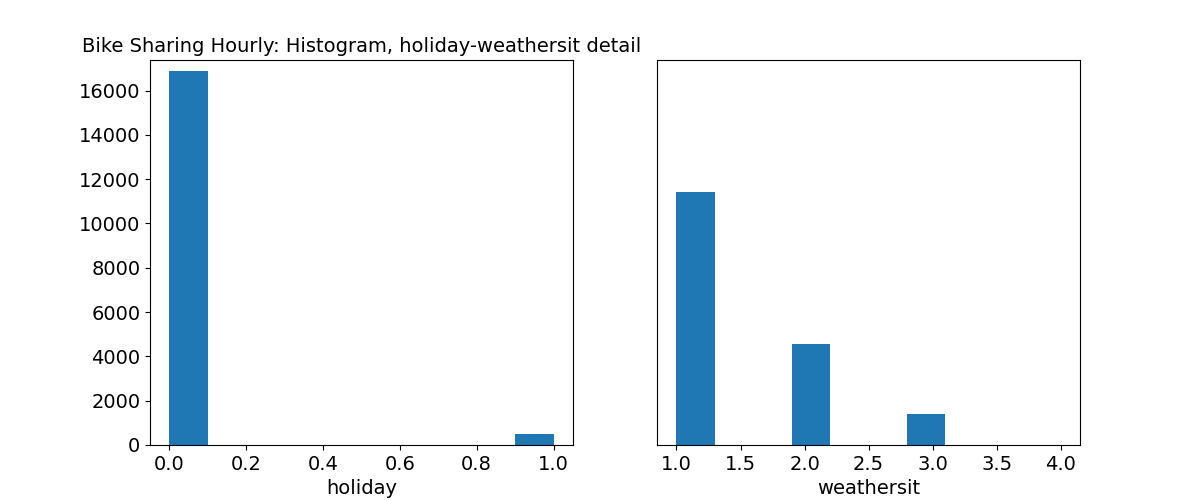
\includegraphics[width=0.7\linewidth]{res/plots/hist_outliers.png}
    \caption{Histograms detail of \textit{holiday} and \textit{weathersit} attributes.}
    \label{fig:hist_detail}
\end{figure}

\subsection{Normal distribution}
The data appears to be normally distributed being plotted in a histogram with number of samples = 1000, mean = 5 and standard deviation = 2

\begin{figure}[H]
    \centering
    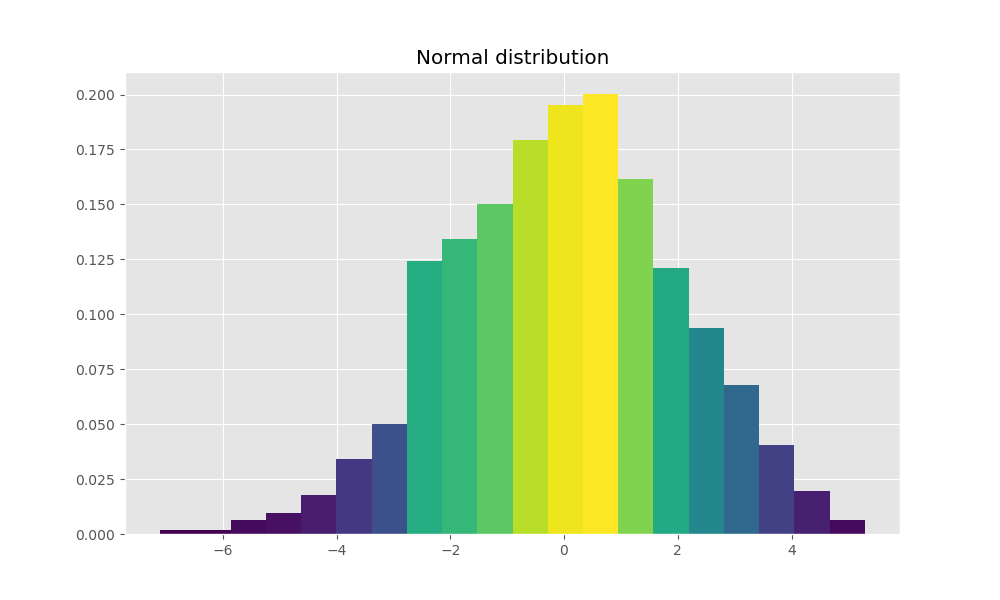
\includegraphics[width=0.6\linewidth]{res/plots/normal_distribution.png}
    \caption{Histogram of the data for normal distribution.}
    \label{fig:normal}
\end{figure}

\subsection{Correlation}

In the following scatter plots, we check for correlation between the $cnt$ attribute and some of the most promising attributes: $season$, $mnth$, $hr$, $weekday$, $workingday$, $weathersit$, $temp$, $atemp$, $hum$, $windspeed$. 

\begin{figure}[H]
    \centering
    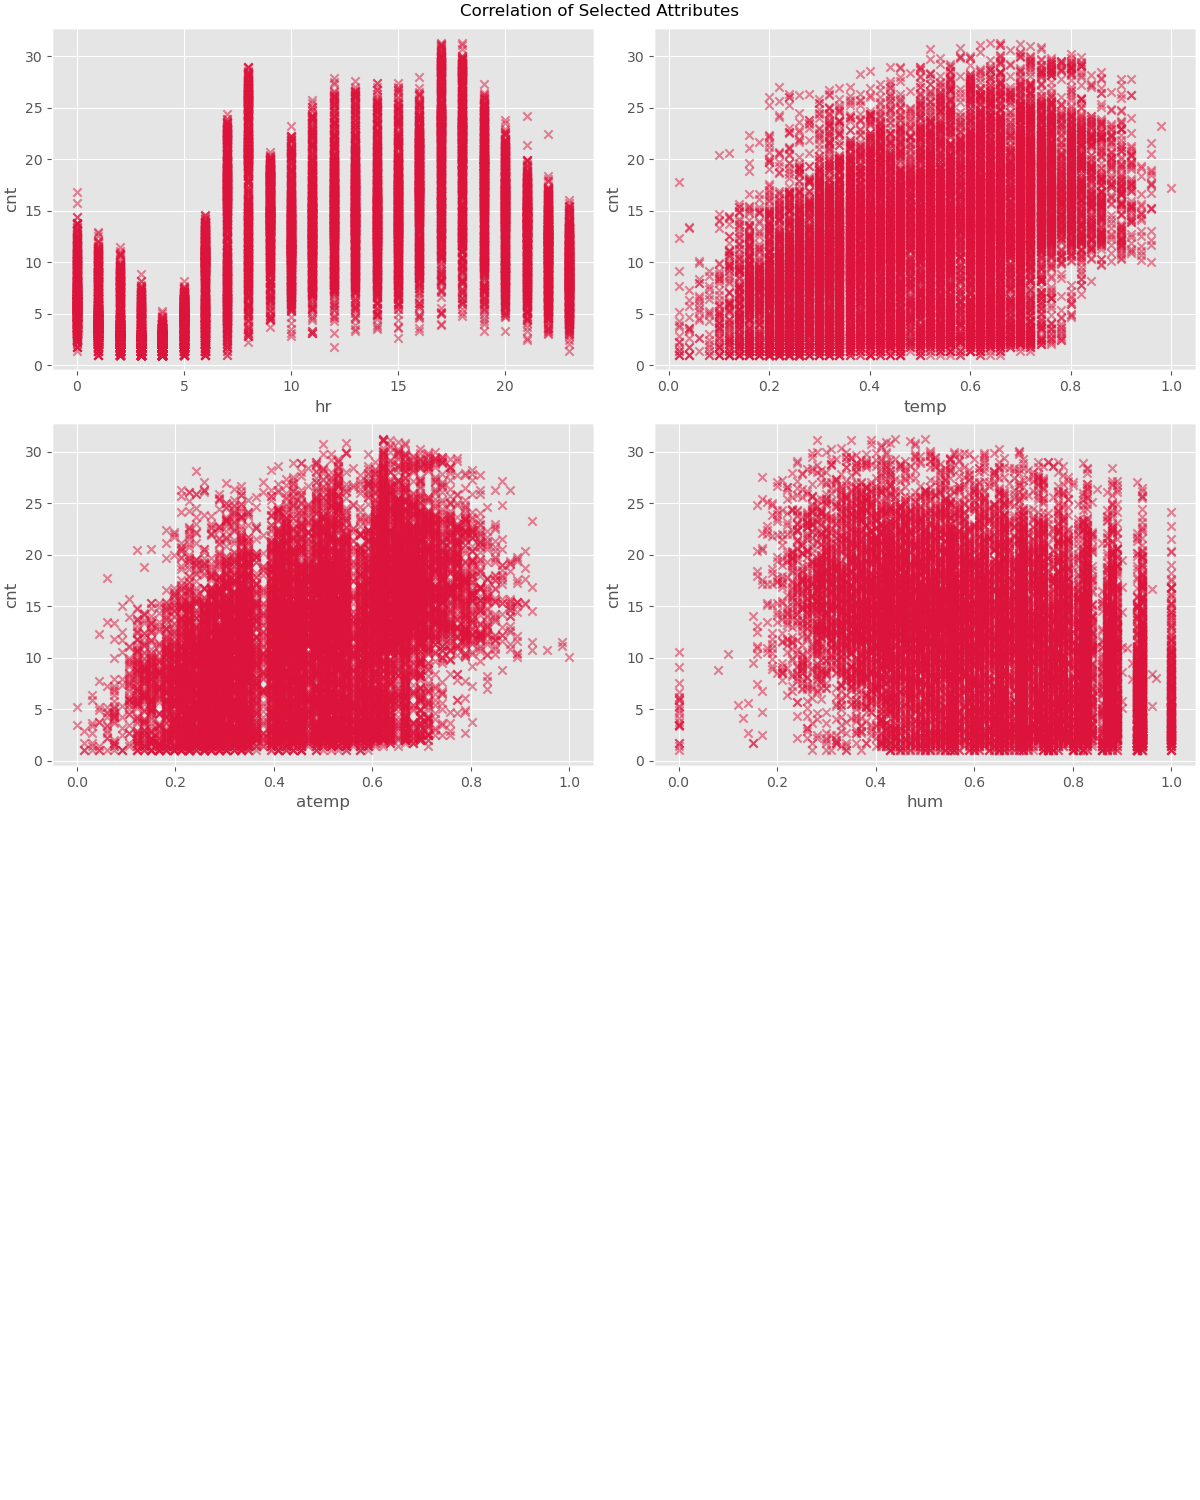
\includegraphics[width=\linewidth]{res/plots/correlation.png}
    \caption{Scatter plots of $cnt$ against other promising attributes.}
    \label{fig:correlation}
\end{figure}


\subsection{Conclusions}

The plots show probable correlation between $cnt$ and most of the other attributes, thus performing regression on $cnt$ as the $y$-variable could bring good results.

% maybe we should also mention classification?  





\section{Conclusion}


\section{Exercises solutions}

\subsection{Question 1}

\paragraph*{Answer:} C.
\paragraph*{Solution:} 
$x_1$ is interval because it describes 30-minute intervals, therefore the distance between one value from the consecutive one is fixed and it has an order since $x_1 = 1$ corresponds to the interval 7:00-7:30, which is sooner in time than the following intervals; $x_6$ is ratio because it's a number and it has a true zero ($x_6 = 0$ means that there are no broken traffic lights); $x_7$ is ratio for the same reason ($x_7 = 0$ means that there are no run over accidents); $y$ is ordinal since it takes values that can be ranked, in this case, from no congestion to a high level of congestion.

\subsection{Question 2}

\paragraph*{Answer:} A
\paragraph*{Solution:} the $\infty$-norm distance between $x_{14}$ and $x_{18}$ is 7.0 because it's indeed the maximum of the absolute value of the differences between the coordinates of the two vectors: max\{|26-19|, |2-0|, 0\} = 7.0


\subsection{Question 3}

\paragraph*{Answer:} A
\paragraph*{Solution:} the variation explained by each principal component is given by $\frac{\sigma_i^2}{\sum_{i'} \sigma_{i'}^2}$, where $\sigma_i$ is the singular value related to the principal component $i$. In this case: $\frac{13.9^2+12.47^2+11.48^2+10.03^2}{13.9^2+12.47^2+11.48^2+10.03^2+9.45^2} = 0,867 > 0,8$

\subsection{Question 4}

\paragraph*{Answer:}
\paragraph*{Solution:} 

\subsection{Question 5}

\paragraph*{Answer:}
\paragraph*{Solution:} 

\subsection{Question 6}

\paragraph*{Answer:}
\paragraph*{Solution:} 


\end{document}

